\begin{Exercise}[title=Effet photoélectrique]
  On envoie sur une photocathode en potassium deux radiation lumineuses; pour une
  radiation ultraviolette $\lambda_1=$\SI{253.7}{nm}, l'énergie des photoélectrons est
  $E_1=3.14eV$ et pour une radiation $\lambda_2=589 nm$ elle vaut $E_2=$\SI{0.36}{eV}
  \begin{center}
    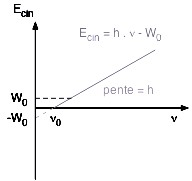
\includegraphics[scale=0.8]{./fig/photoel.jpg}
  \end{center}
  \Question Déterminer la constante de Planck $h$
  \Question Déterminer l'énergie d'extraction $W$ des électrons pour le potassium.
  \Question Calculer la longueur d'onde maximale du rayonnement produisant un
  effet photoélectrique sur le potassium.
\end{Exercise}
\begin{Answer}
  \Question  $E_i= \frac{hc}{\lambda_i}+W$ donc :
  \[h= \frac{\lambda_1\lambda_2}{\lambda_2-\lambda_1}(\frac{E_2-E_1}{c}\]
  \Question directement avec la formule
  \Question directement avec la formule
\end{Answer}
